\documentclass[11pt, titlepage,a4paper]{article}
\usepackage[utf8]{inputenc}
\usepackage{natbib}
\usepackage{hyperref}
\usepackage{dsfont}
\usepackage{subfigure}
\usepackage{multicol}
\usepackage[T1]{fontenc}
\usepackage[left=2cm,right=2cm,top=2cm,bottom=2cm]{geometry}
\usepackage[spanish, activeacute]{babel}
\usepackage{amsmath}
\usepackage{amssymb,amsfonts,textcomp}
\usepackage{color}
\usepackage{array}
\usepackage{hhline}
\usepackage{varwidth}
\usepackage{graphicx}
\usepackage{parcolumns}
\usepackage{cite}
\usepackage{hyperref}
\usepackage[]{algorithm2e}


\hypersetup{ colorlinks=true, linkcolor=black, citecolor=black, filecolor=black,
urlcolor=blue, pdftitle=Laboratorio 6: Clustering Jerarquico , pdfauthor= Alberto Fernández Arkaitz Marcos Endika Serrano}


\renewcommand{\thefootnote}{\fnsymbol{footnote}}
\title{\textbf{\huge{Mineria de Datos} \\Laboratorio 6: Clustering
Jerarquico \newline
\begin{center}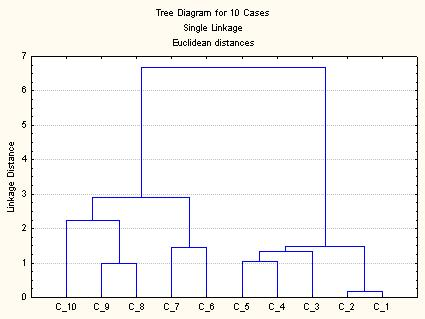
\includegraphics[scale =
1.4]{./images/Portada.jpg}\newline\footnote{Imagen extraida de
\url{http://jmj-qa.blogspot.com.es/2011/09/analisis-cluster.html}}\end{center}}
}
%\title{\begin{center}\textbf{\Huge{Sistemas de Apoyo a la Decisión} \newline
% \newline Práctica 2: Clasificación k-NN} \newline \begin{center}\includegraphics{./img/220px-KnnClassification.png}\footnote{Imagen extraida de \url{http://es.wikipedia.org/wiki/Knn}}\end{center} \newline 
%\end{center}}

\author{Alberto Fernández \and Arkaitz Marcos \and Endika Serrano}
\date{}
\bibliographystyle{alpha}

\begin{document}
\maketitle

\tableofcontents

\newpage
\renewcommand{\thefootnote}{\arabic{footnote}}
\section{Introducción}

\subsection{Definición}
\cite{Witten}
\subsection{Objetivo}

\section{Algoritmo}
%Clustering jerarquico en pseudocodigo
\begin{algorithm}[H]
 \KwData{Las instancias que se quieren }
 \KwResult{Las tablas agrupando los datos en clusters}
 
 Carga del fichero arff
 \While{not at end of this document}{
  read current\;
  \eIf{understand}{
   go to next section\;
   current section becomes this one\;
   }{
   go back to the beginning of current section\;
  }
 }
 \caption{How to write algorithms}
\end{algorithm}

\section{Diseño}
%Diagrama de clases

\section{Resultados experimentales}

\subsection{Banco de pruebas}

\subsection{Resultados obtenidos}

\subsection{Resultados respecto a otro software}

\subsection{Análisis de resultados}

\subsection{Rendimiento del software}

\section{Conclusiones}

\section{Bibliografía}
%Con estos comandos obtenemos todas las referencias bibliogr�ficas que se hacen
% en el texto, obtenidas en las BD que le indicamos en el siguiente comando, se pueden indicar m�s de una BD, separadas por comas.
%\bibliography{bibliografia}

\section{Valoración subjetiva}
\bibliography{bibliografia}

\end{document}